\begin{figure}[t]
\centering
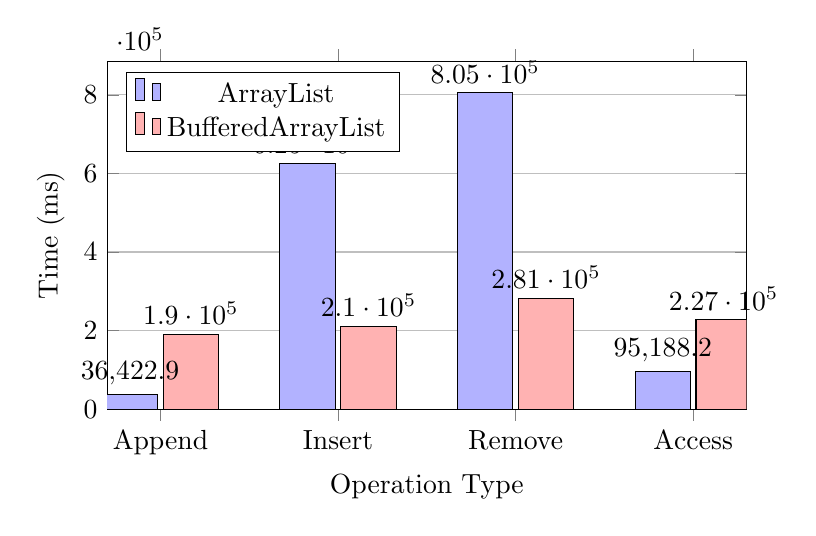
\begin{tikzpicture}
\begin{axis}[
    width=0.8\columnwidth,
    height=6cm,
    xlabel={Operation Type},
    ylabel={Time (ms)},
    ybar,
    bar width=20pt,
    symbolic x coords={Append,Insert,Remove,Access},
    xtick=data,
    nodes near coords,
    nodes near coords align={vertical},
    legend pos=north west,
    ymajorgrids=true,
    ymin=0,
]

\addplot[fill=blue!30] coordinates {
    (Append,36422.9)
    (Insert,624778.9)
    (Remove,805294.5)
    (Access,95188.2)
};

\addplot[fill=red!30] coordinates {
    (Append,190340.1)
    (Insert,209963.8)
    (Remove,281027.1)
    (Access,227419.3)
};

\legend{ArrayList,BufferedArrayList}

\end{axis}
\end{tikzpicture}
\caption{Performance comparison between ArrayList and BufferedArrayList for different operations (100K elements)}
\label{fig:performance}
\end{figure} 